\documentclass[12pt,a4paper]{article}
\usepackage{amsmath,amscd,amsbsy,amssymb,latexsym,url,bm,amsthm}
\usepackage{epsfig,graphicx,subfigure}
\usepackage{enumitem,balance}
\usepackage{wrapfig}
\usepackage{mathrsfs,euscript}
\usepackage[usenames]{xcolor}
\usepackage{hyperref}
\usepackage[vlined,ruled,linesnumbered]{algorithm2e}
\hypersetup{colorlinks=true,linkcolor=black}

\newtheorem{theorem}{Theorem}
\newtheorem{lemma}[theorem]{Lemma}
\newtheorem{proposition}[theorem]{Proposition}
\newtheorem{corollary}[theorem]{Corollary}
\newtheorem{exercise}{Exercise}
\newtheorem*{solution}{Solution}
\newtheorem{definition}{Definition}
\theoremstyle{definition}

\renewcommand{\thefootnote}{\fnsymbol{footnote}}

\newcommand{\postscript}[2]
 {\setlength{\epsfxsize}{#2\hsize}
  \centerline{\epsfbox{#1}}}

\renewcommand{\baselinestretch}{1.0}

\setlength{\oddsidemargin}{-0.365in}
\setlength{\evensidemargin}{-0.365in}
\setlength{\topmargin}{-0.3in}
\setlength{\headheight}{0in}
\setlength{\headsep}{0in}
\setlength{\textheight}{10.1in}
\setlength{\textwidth}{7in}
\makeatletter \renewenvironment{proof}[1][Proof] {\par\pushQED{\qed}\normalfont\topsep6\p@\@plus6\p@\relax\trivlist\item[\hskip\labelsep\bfseries#1\@addpunct{.}]\ignorespaces}{\popQED\endtrivlist\@endpefalse} \makeatother
\makeatletter
\renewenvironment{solution}[1][Solution] {\par\pushQED{\qed}\normalfont\topsep6\p@\@plus6\p@\relax\trivlist\item[\hskip\labelsep\bfseries#1\@addpunct{.}]\ignorespaces}{\popQED\endtrivlist\@endpefalse} \makeatother

\begin{document}
\noindent

%========================================================================
\noindent\framebox[\linewidth]{\shortstack[c]{
\Large{\textbf{Lab02-Divide and Conquer}}\vspace{1mm}\\
CS214-Algorithm and Complexity, Xiaofeng Gao, Spring 2021.}}
\begin{center}
\footnotesize{\color{red}$*$ If there is any problem, please contact TA Haolin Zhou. }

\footnotesize{\color{blue}$*$ Name:Yanjie Ze  \quad Student ID:519021910706 \quad Email: zeyanjie@sjtu.edu.cn}
\end{center}

\begin{enumerate}
\item
    \textit{Recurrence examples.} Give asymptotic upper and lower bounds for $T(n)$ in each of the following recurrences. Assume that $T(n)$ is constant for sufficiently small $n$. Make your bounds as tight as possible.
\begin{enumerate}
	\item $T(n)=4 T(n / 3)+n \log n$
	\item $T(n)=4 T(n / 2)+n^{2} \sqrt{n}$
	\item $T(n)=T(n-1)+n$	
	\item $T(n)=2T(\lfloor \sqrt n\rfloor)+\log n$
\end{enumerate}
\begin{solution}
\begin{enumerate}
% 第一题
\item 
$$
a=4, b=3, log_ba=log_34
$$
Since $n<nlogn<n^2$, and based on Master Theorem, we have:
$$
T(n)=O(n^2), T(n)=\Omega(n^{log_34})
$$

\item
 $$
 T(n)=4 T(n / 2)+n^{2} \sqrt{n}=4 T(n / 2)+n^{\frac{5}{2}} 
 $$
 Based on Master Theorem, $a=4, b=2, log_ba=2, d=\frac{5}{2}$,we have:
 
 $$
 T(n) = \Theta(n^\frac{5}{2})
 $$
 
 \item
 $$
 \displaystyle T(n)=\sum_{i=1}^ni+T(0) = \frac{n^2+n}{2}+T(0)
 $$
 Thus:
 $$
 T(n)=\Theta(n^2)
 $$
 
 \item
Assume $n=2^{2^k}$, then $k=log_2(log_2n)$. 

$$
T(2^{2^k}) = 2T(2^{2^{k-1}})+2^klog2
$$
$$
\frac{T(2^{2^k})}{2^k} = \frac{T(2^{2^{k-1}})}{2^{k-1}}+log2
$$
Thus we can sum them together and get:
$$
 \frac{T(2^{2^k})}{2^k} = (k-1)log2 + T(2)
$$
Multiply both sides by $2^k$ and then replace $k$ by $n$:
$$
T(n) = log2\cdot log_2n\cdot log_2(log_2n)+ T(2)\cdot log_2n
$$
Therefore:
$$
T(n) = \Theta(logn\cdot log(logn))
$$

\end{enumerate}
\end{solution}
\item
\textit{Divide-and-conquer.} Given an integer array $A[1..n]$ and two integers $lower \le upper$, design an algorithm using \textbf{divide-and-conquer} method to count the number of ranges $(i,j)$ ($1 \leq i \leq j \leq n$) satisfying
$$
    lower \leq \sum_{k=i}^{j}{A[k]} \leq upper.
$$
\textbf{Example:}

Given $A = [1,-1,2]$, $lower = 1$, $upper = 2$, return 4.

The resulting four ranges are $(1,1)$, $(3,3)$, $(2,3)$ and $(1,3)$.

\begin{enumerate}
\item
Complete the implementation in the provided C/C++ source code {\color{blue}(The source code \emph{Code-Range.cpp} is attached on the course webpage)}.
\item
Write a recurrence for the running time of the algorithm and solve it by recurrence tree {\color{blue}(You can modify the figure sources \emph{Fig-RecurrenceTree.vsdx} or \emph{Fig-RecurrenceTree.pptx} to illustrate your derivation)}.
\item
Can we use the Master Theorem to solve the recurrence above? Please explain your answer.
\end{enumerate}

%第二题
\begin{solution}
\begin{enumerate}
\item
Code is in \textbf{Code-Range.cpp}.
\item
The recurrence is:
$$
T(n) = 2T(\frac{n}{2}) + nlogn
$$
And the recurrence tree is:
\begin{figure}[htbp]
    \centering
    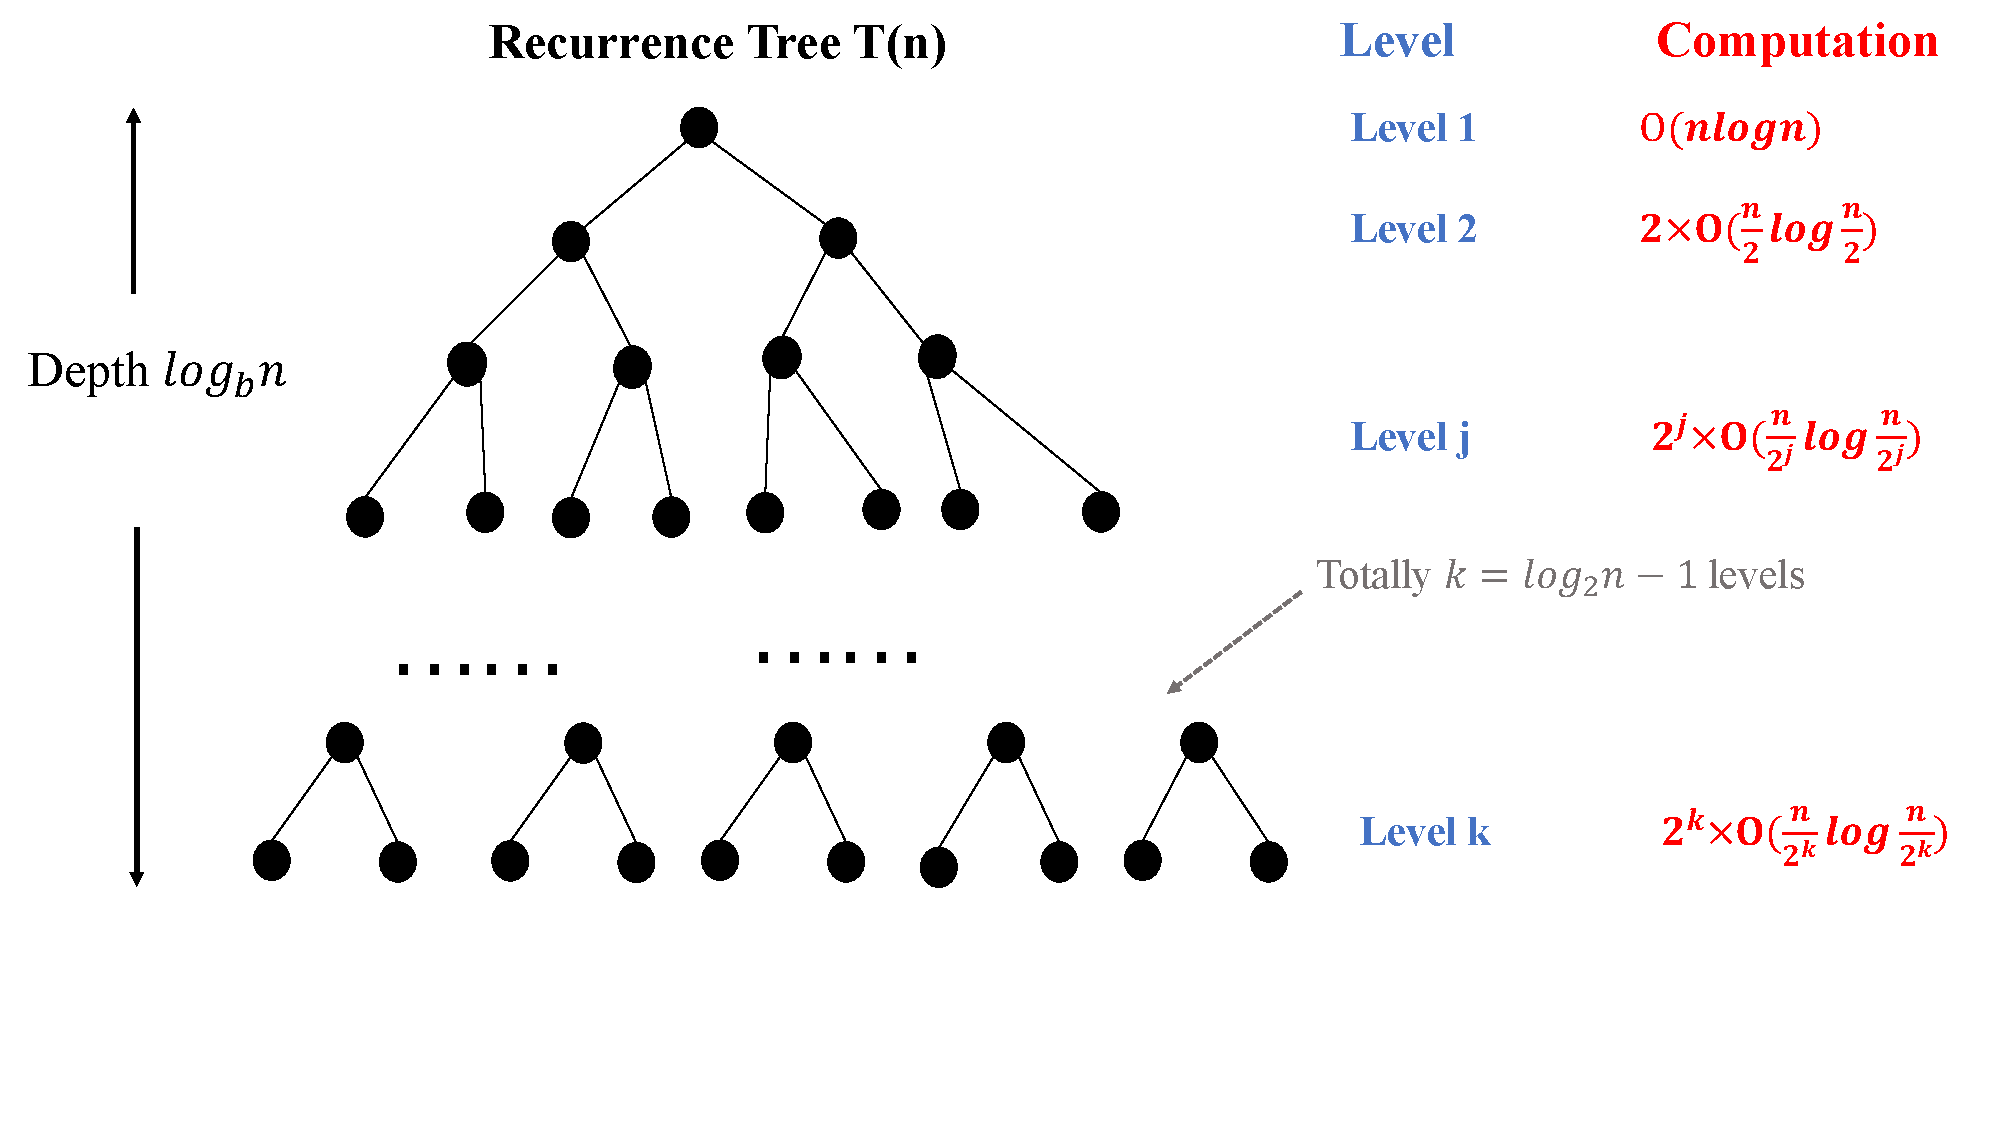
\includegraphics[width=0.6\textwidth]{Fig-RecurrenceTree.pdf}
    \caption{A Recurrence Tree}\label{Fig-RecurrenceTree}
\end{figure}


Then we calculate the sum:
$$
\displaystyle T(n) = \sum_{i=1}^{log_2n-1}2^i\times O(\frac{n}{2^i}log\frac{n}{2^i})
$$
After the simplification we get:
$$
\displaystyle T(n) = n\sum_{i=1}^{log_2n-1}(O(logn)-ilog2)
$$
Thus:
$$
\displaystyle T(n)=n\left((log_2n-1)O(logn) - \frac{logn(log_2n-1)}{2}\right)
$$
Which means:
$$
T(n) = O(n\log^2 n)
$$

\item
We denote:
$$
a=2,b=2,\log_ba=1
$$
Since $nlogn=O(n^2)$, we can have the bound based on the master theorem:
$$
T(n)=O(n^2)
$$
Which is not tight.

However, from Wikipedia and CLRS we can know that there is a more advanced version of master theorem, which can explain this recurrence.
$$
If\ f(n)=\Theta(n^{log_ba}log^kn),k\geq 0, then\ T(n)=\Theta(n^{log_ba}log^{k+1}n).
$$
Thus:
$$
T(n)=\Theta(n^{\log_ba}log^2n)=\Theta(n\log^2n)
$$


\end{enumerate}
\end{solution}
\item
\textit{Transposition Sorting Network.} A comparison network is a \textbf{transposition network}  if each comparator connects adjacent lines, as in the network in Fig. ~\ref{Fig-Transposition}.

\begin{figure}[htbp]
    \centering
    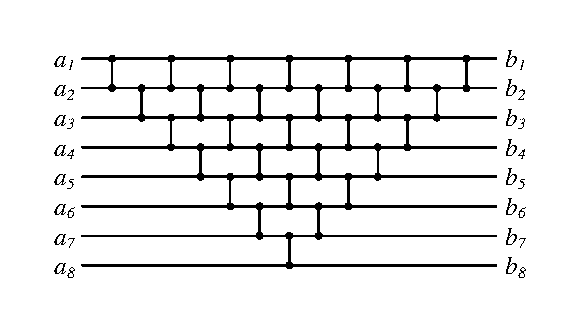
\includegraphics[width=0.4\textwidth]{Fig-Transposition.pdf}
    \caption{A Transposition Network Example}\label{Fig-Transposition}
\end{figure}

\begin{enumerate}
\item Prove that a transposition network with $n$ inputs is a sorting network if and only if it sorts the sequence $\langle n, n-1, \cdots, 1 \rangle$. {\color{blue}(Hint: Use an induction argument analogous to the \emph{Domain Conversion Lemma}.)}
\item {\color{red}{(Optional Sub-question with Bonus)}} Given any $n \in \mathbb{N}$, write a program using Tkinter in Python to draw a figure similar to Fig.~\ref{Fig-Transposition} with $n$ input wires.
\end{enumerate}


\begin{solution}
\begin{enumerate} 
\item
~\\
\textbf{After I think through this problem, I try my best to figure out a proof, which is somewhat not rigorous. And after I discuss the problem with my classmates I also get a solution which is rigorous. Anyway, I consider my own solution is directer, and another solution is rigorous but not that direct. Finally I decide to just keep my original solution, and the rigorous one is referred in the appendix~\ref{solution}.}

~\\


First, it is obvious that if a transposition network is a sorting network, it can sort the sequence $\langle n, n-1, \cdots, 1 \rangle$. 

Second, we will prove if a transposition network sorts the sequence $\langle n, n-1, \cdots, 1 \rangle$, it is a sorting network.

\textbf{Proof:}\\

\textbf{Basic step:}\\

\textbf{When n=3}, the network can sort $\langle 3, 2, 1 \rangle$. Since the biggest number is on the top, to transfer it to the bottom, we need at least 2 comparators. After transferring the top one, the rest of the numbers need one more comparator so that the smaller one can be transferred to the top. Therefore, we finally get the network which can sort this sequence in Fig.~\ref{s3}.\\

Though the more comparators can be added to this network without influencing the sort ability, the architecture in Fig.~\ref{s3} is the simplest one, and more comparators are meaningless since they will do no exchange when comparing.\\



\begin{figure}[htbp]
    \centering
    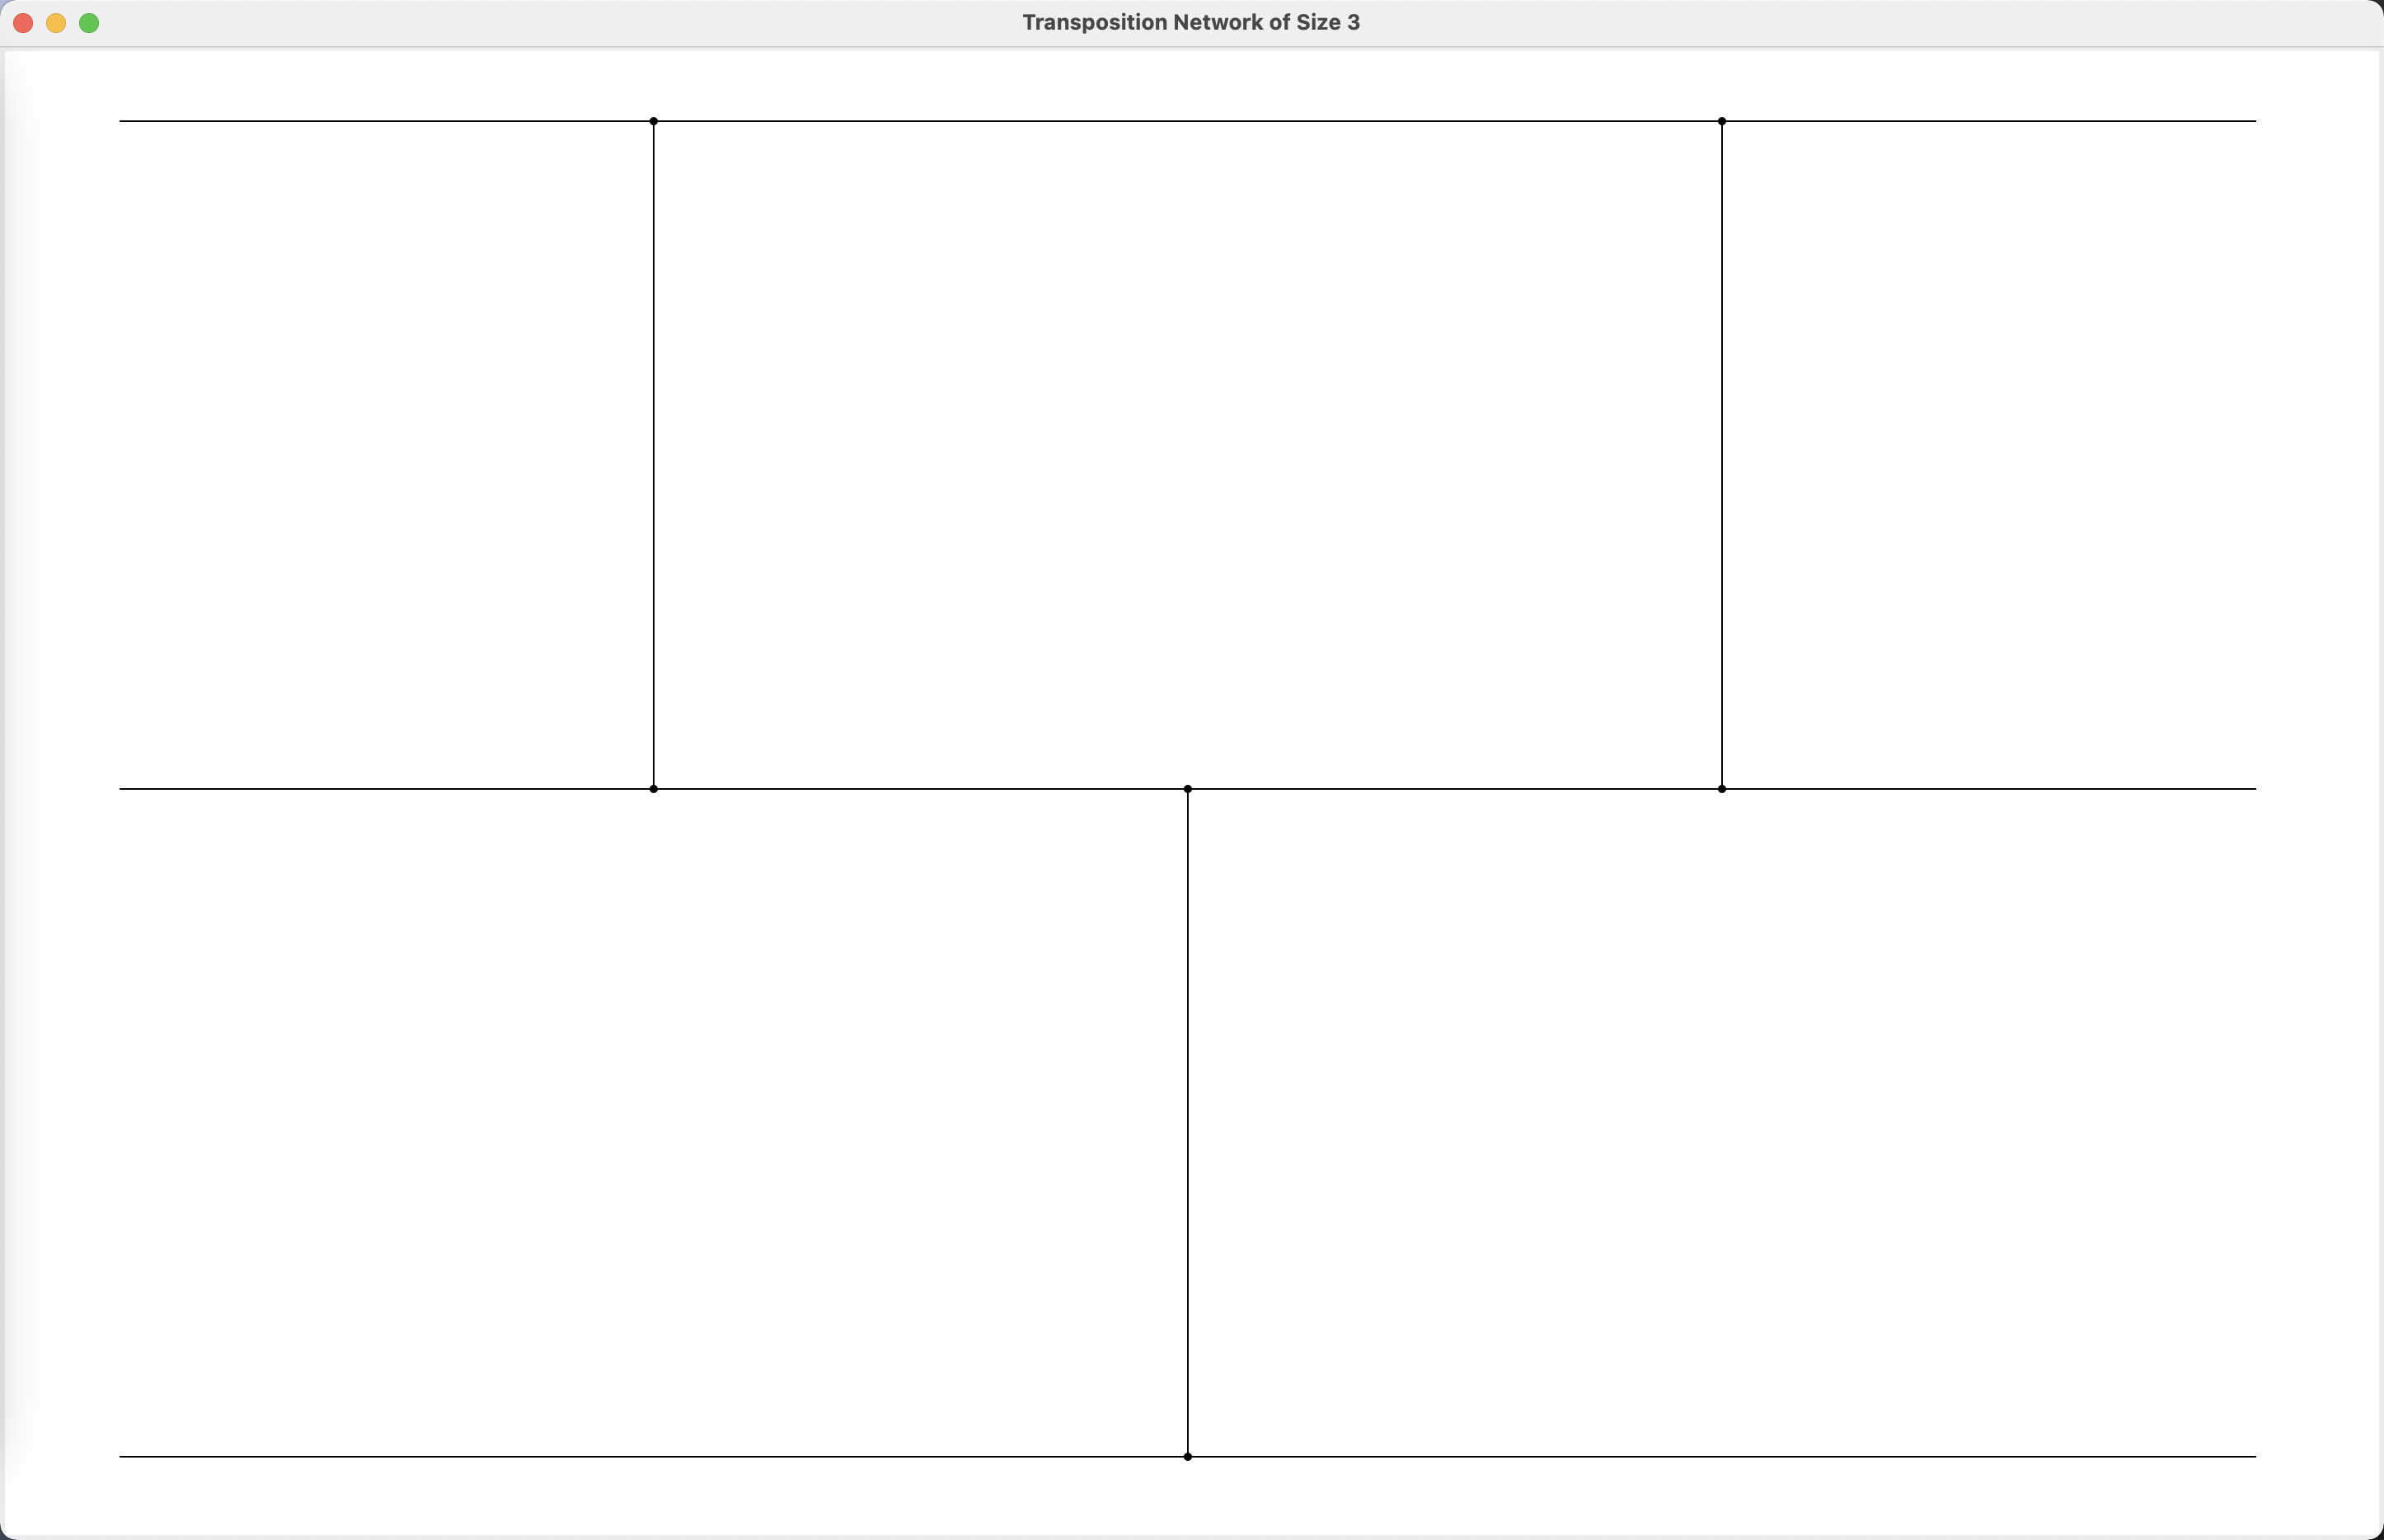
\includegraphics[width=0.6\textwidth]{size3.png}
    \caption{A Transposition Network of size 3}\label{s3}
\end{figure}

Now the problem is: Is this architecture a sorting network?

The answer is YES.

This network essentially can be seen as a \textbf{bubble sort}. Two adjacent elements are compared by a comparator and the smaller one is on top then, which is one bubble. Therefore, this network works the same as \textbf{bubble sort}, which proves it can function as a sorting network.

Therefore, we finish the basic step of proof, and here is the conclusion:

\textbf{The network can sort} $\langle 3, 2, 1 \rangle$ $\Rightarrow$ \textbf{The network's simplest architecture has the shape in Fig.}~\ref{s3} $\Rightarrow$ \textbf{The network is a sorting network.}

~\\
\textbf{Induction Hypothesis:}

Assume for $n\leq k$, if the network can sort $\langle k, k-1, ..., 1\rangle$, then the network's simplest architecture has the shape in Fig.~\ref{s6}.

(Because the network for $n=k$ is hard to draw, we use $n=6$ for $n=k$ and $n=7$ for $n=k+1$.)

\begin{figure}[htbp]
    \centering
    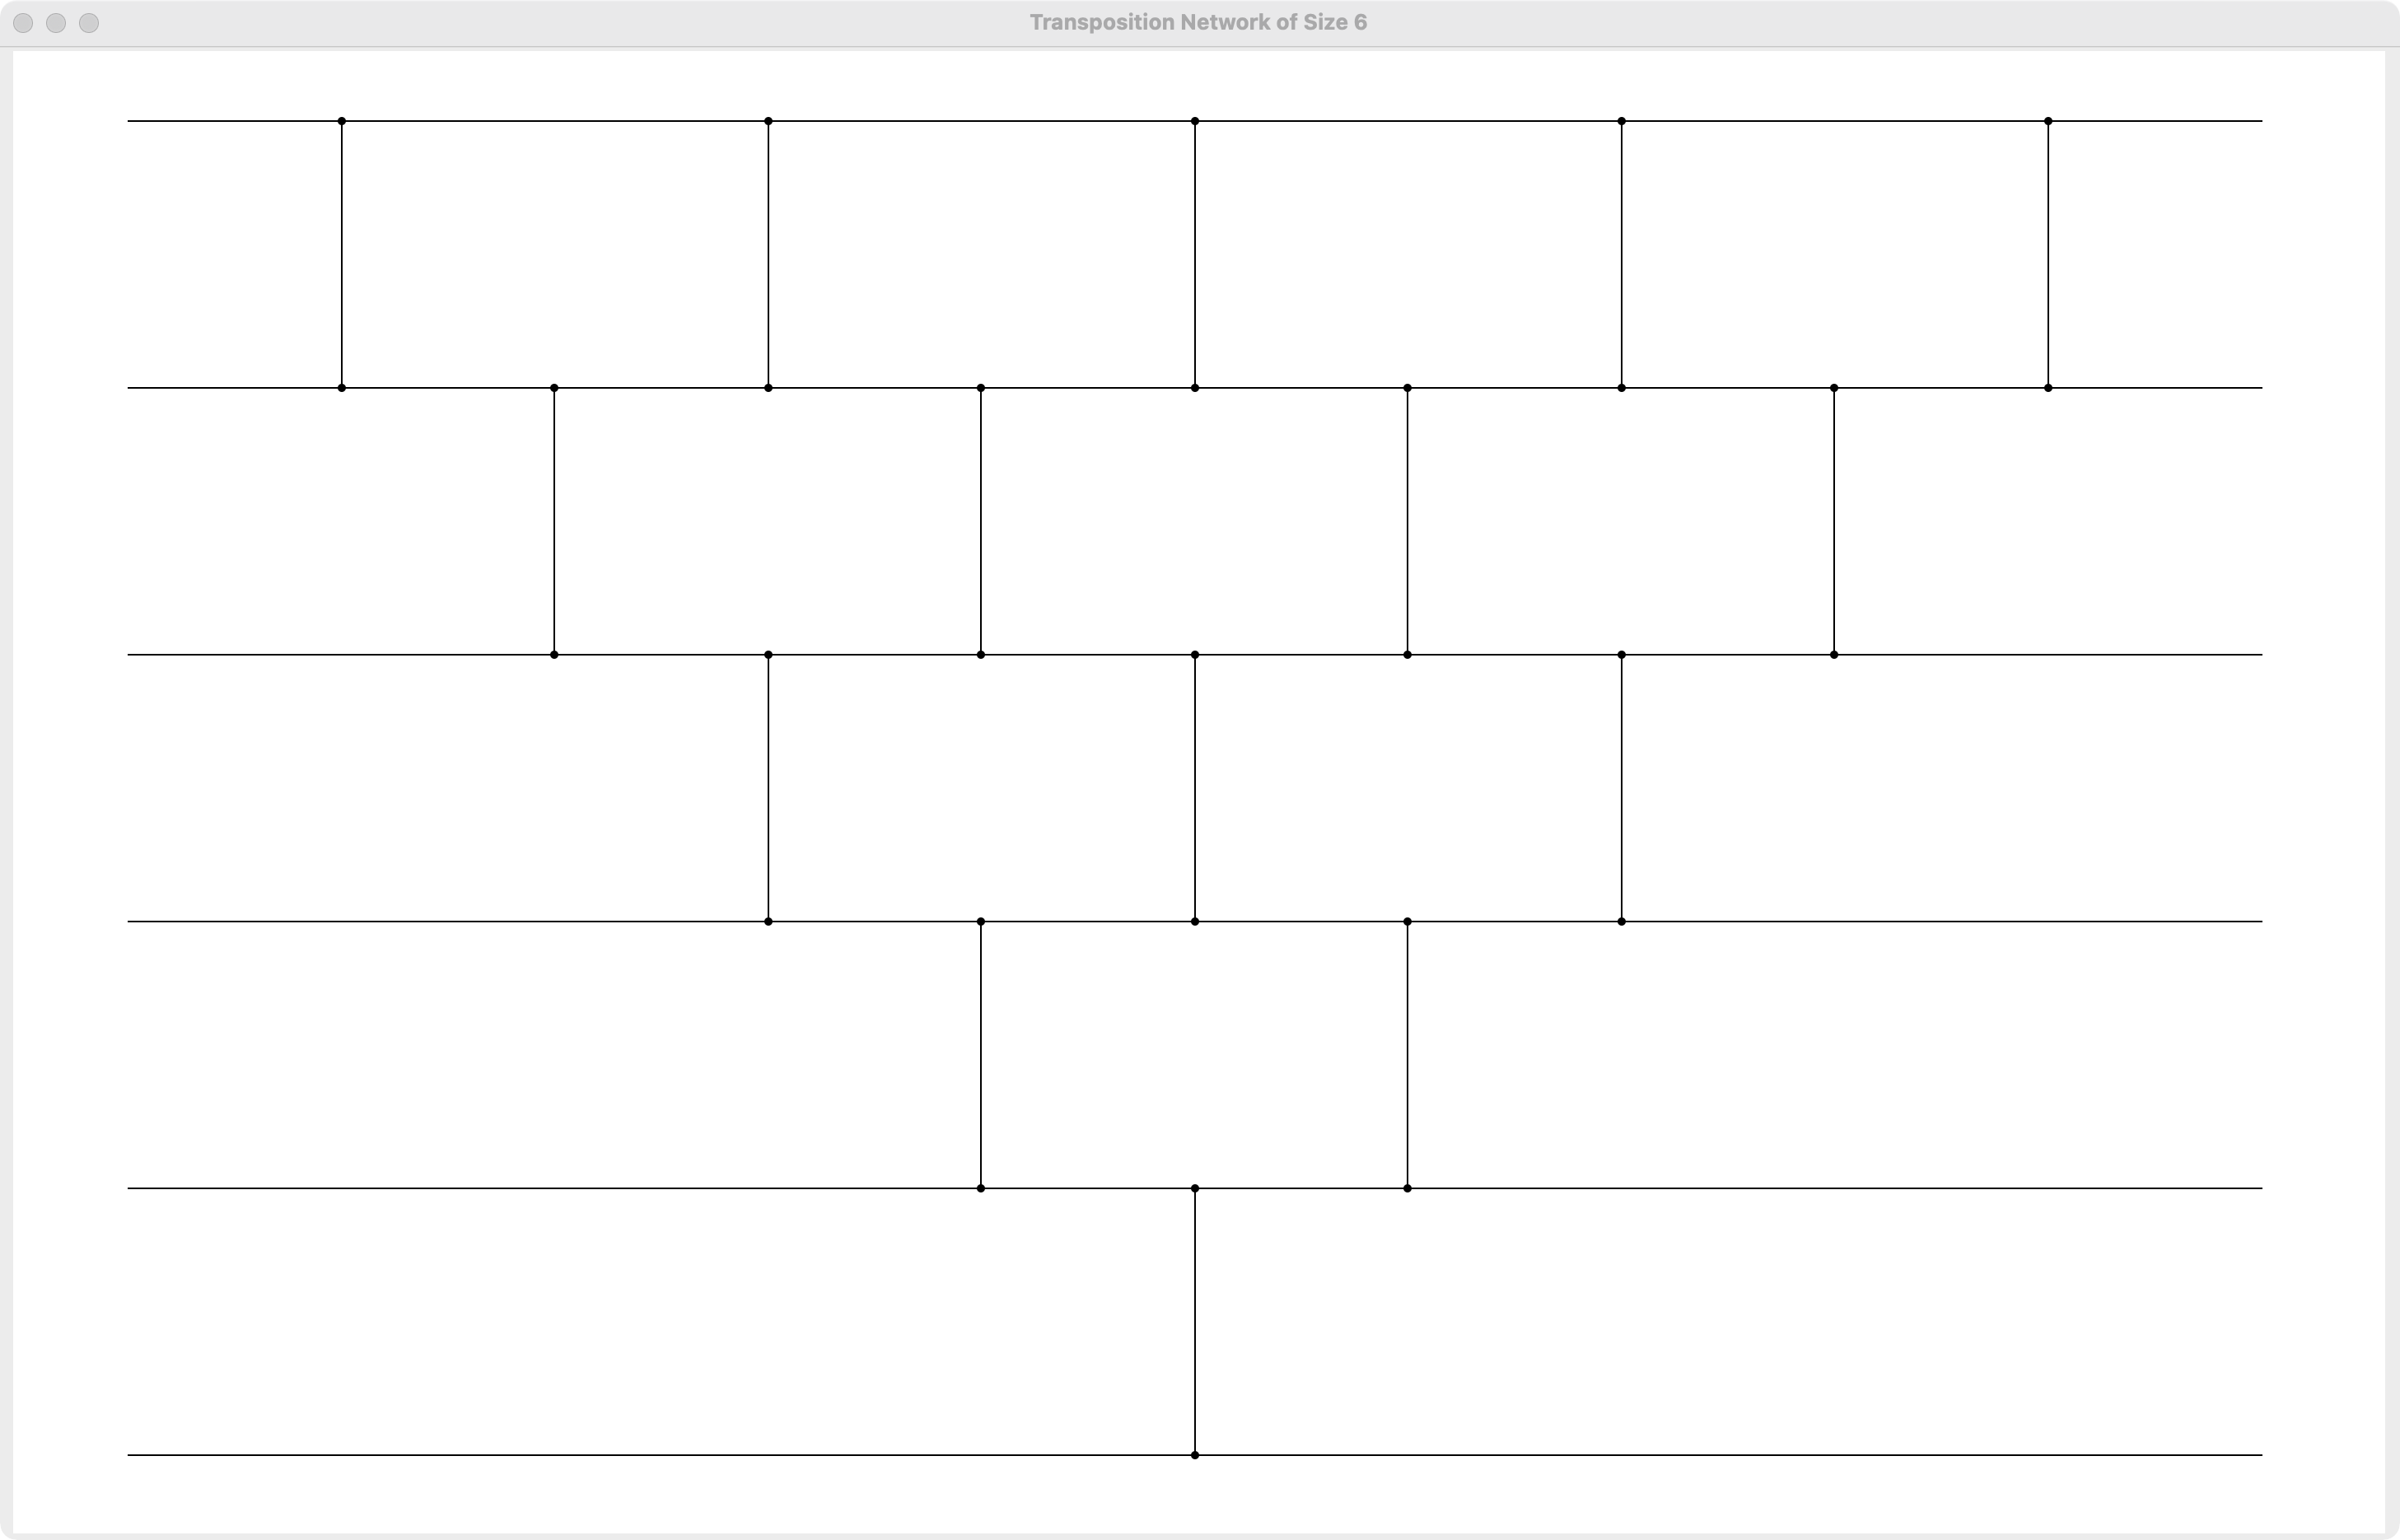
\includegraphics[width=0.6\textwidth]{size6.png}
    \caption{A Transposition Network of size 6}\label{s6}
\end{figure}

~\\
\textbf{Proof of Induction Step:}We prove: for $n=k+1$, if the network can sort $\langle k+1, k, ..., 1\rangle$, then the network's simplest architecture has the shape in Fig.~\ref{s7}.


\begin{figure}[htbp]
    \centering
    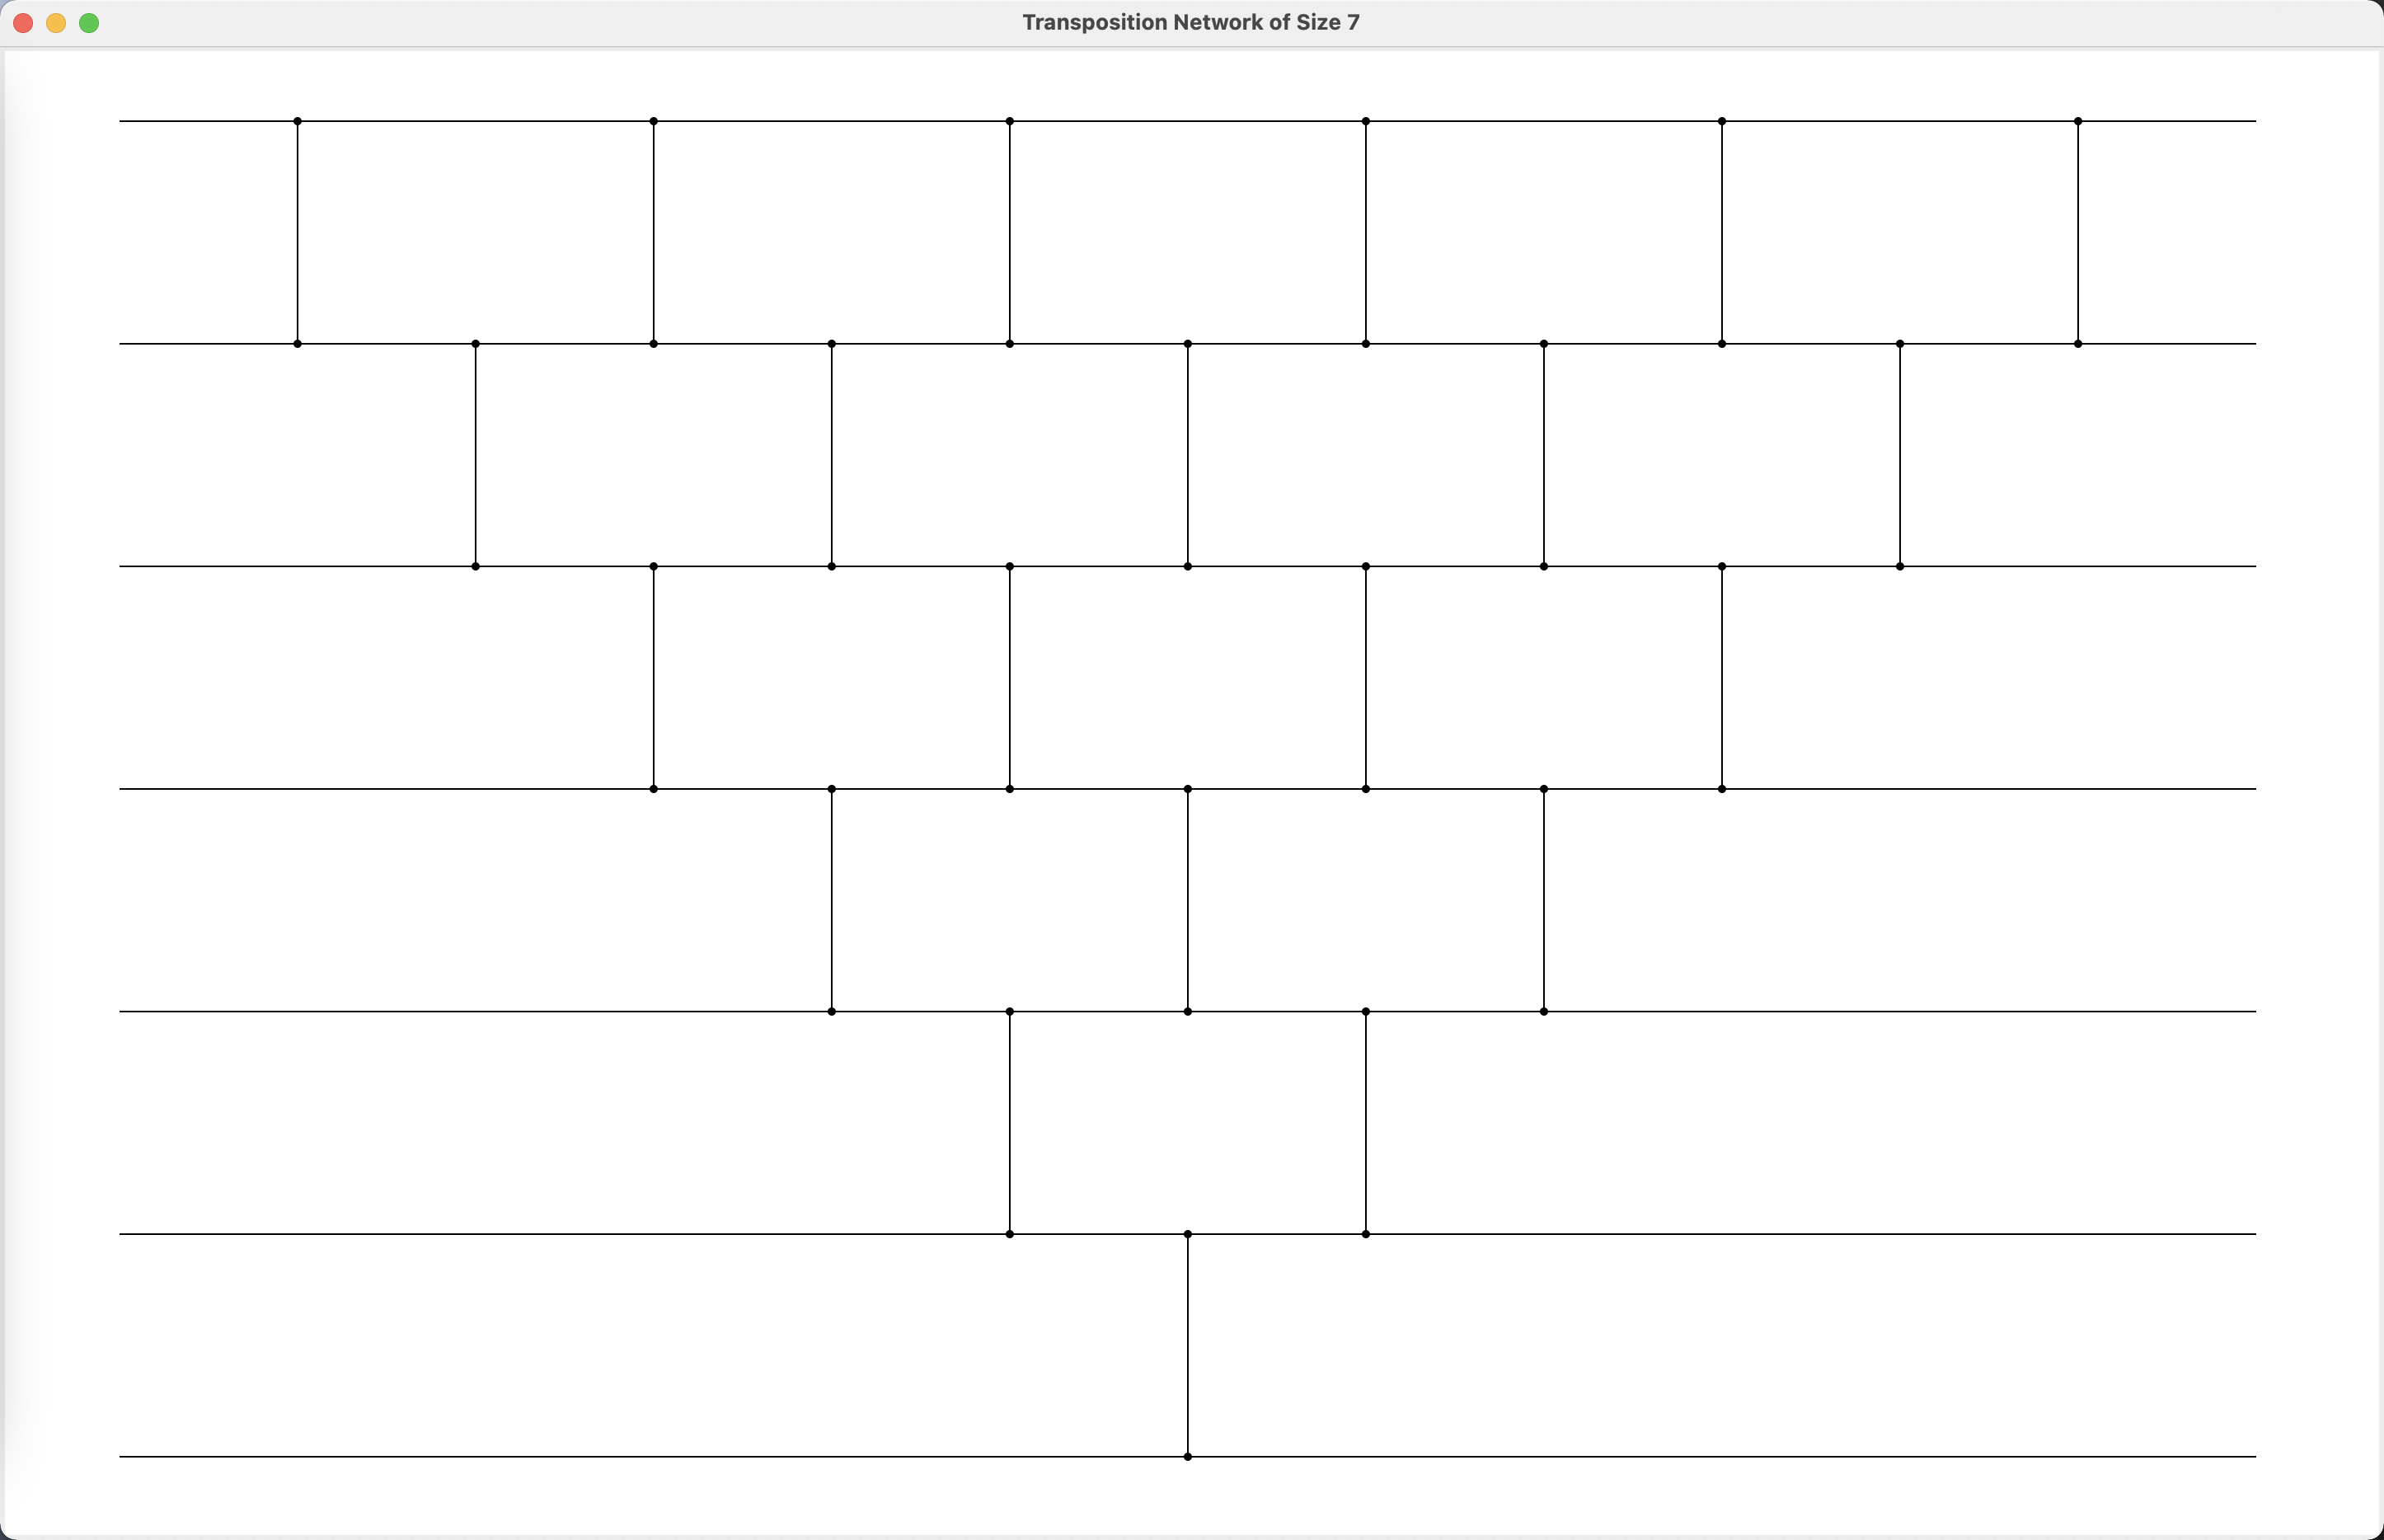
\includegraphics[width=0.6\textwidth]{size7.png}
    \caption{A Transposition Network of size 7}\label{s7}
\end{figure}


When $n\leq k$, the network has been a sorting network, which means for the input $\langle k+1, k, ..., 2, 1\rangle$, $\langle k+1, k, ..., 2\rangle$ can be sorted correctly. 

Then for the element $1$ at the bottom, to make it sorted correctly, the element should be transferred to the top, which means this element at least goes through $k$ times of bubble, or $k$ comparators. 

If the comparators' number is less than $k$, then the element can not be transferred to the top.

If the comparators' number is more than $k$, then the element can  be transferred to the top, but the extra comparators are useless.

Therefore, to make the bottom element sorted correctly, the network's simplest architecture has the shape in Fig.~\ref{s7}.

Finally, we prove that for $n=k+1$, if the network can sort $\langle k+1, k, ..., 1\rangle$, then the network's simplest architecture has the shape in Fig.~\ref{s7}.

And this means if the network can sort $\langle k+1, k, ..., 1\rangle$, then the network is a sorting network, which is proved before.


\item
Code is in \textbf{sorting\_network.py}.

Fig.~\ref{s6}, Fig.~\ref{s7}, Fig.~\ref{s100}, Fig.~\ref{s300} are  all drawn by the program.



\begin{figure}[htbp]
    \centering
    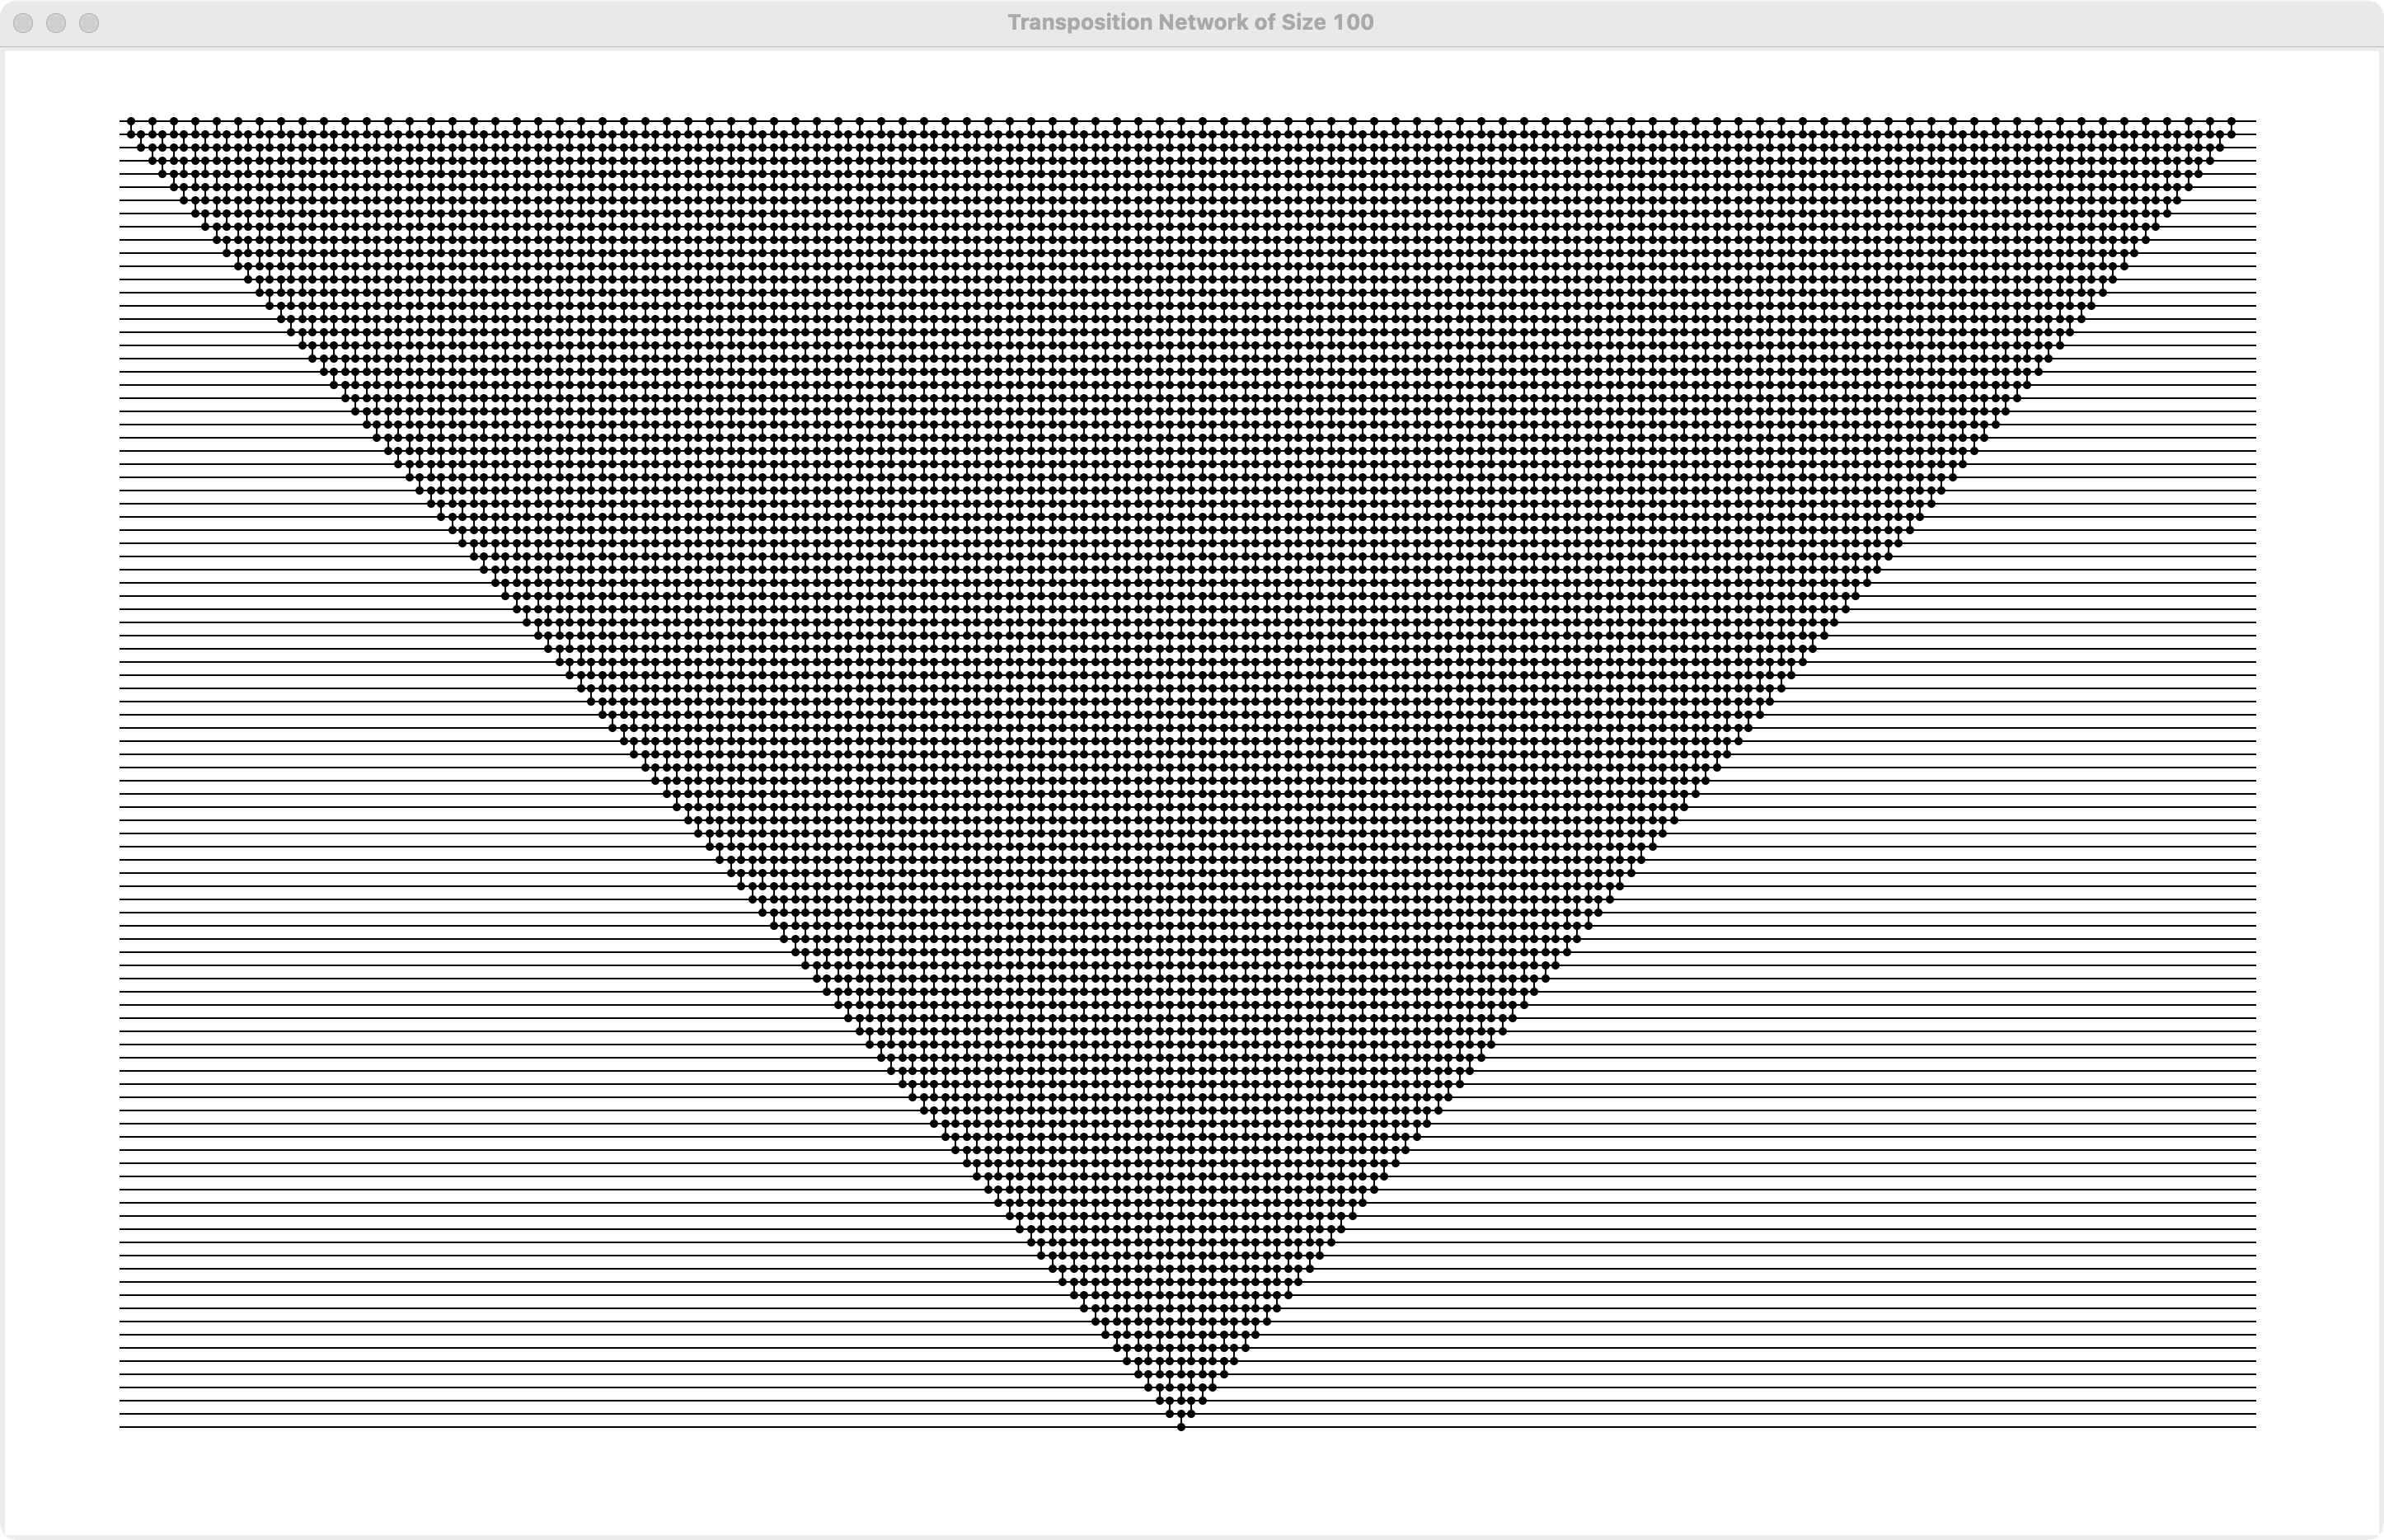
\includegraphics[width=0.6\textwidth]{size100.png}
    \caption{A Transposition Network of size 100}\label{s100}
\end{figure}

\begin{figure}[htbp]
    \centering
    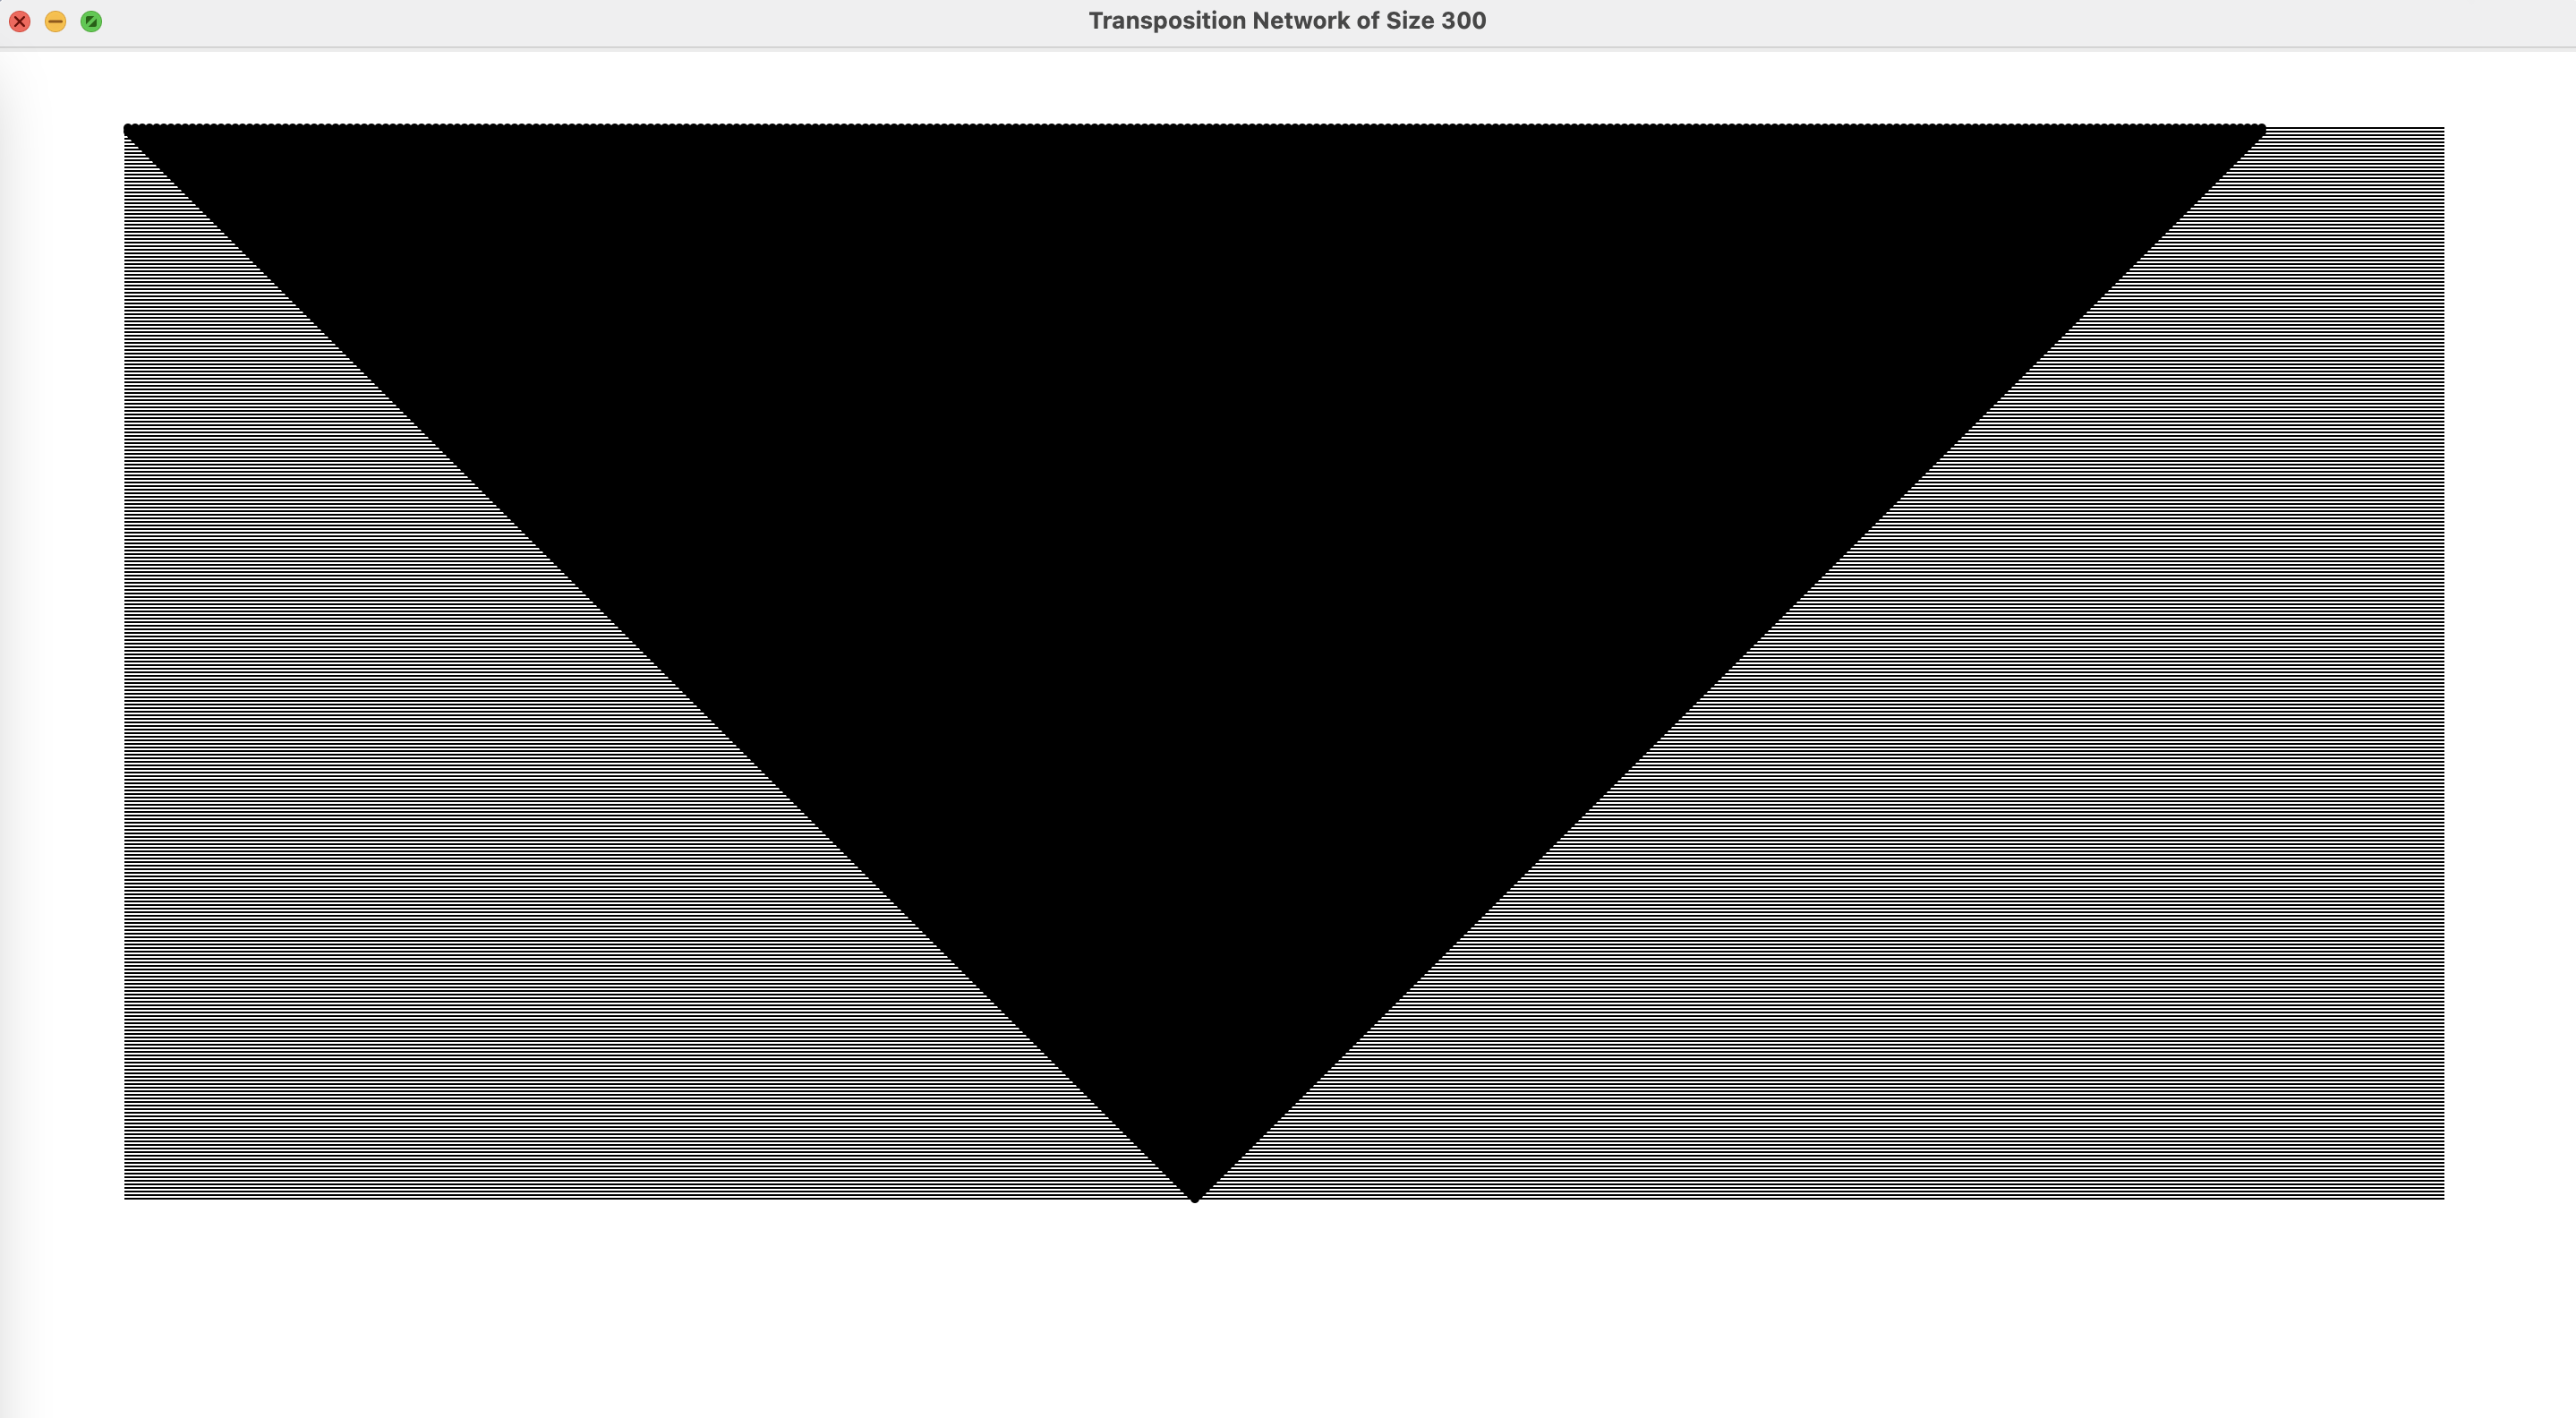
\includegraphics[width=0.6\textwidth]{size300.png}
    \caption{A Transposition Network of size 300}\label{s300}
\end{figure}

\end{enumerate}
\end{solution}
\section*{Appendix}
\begin{figure}[htbp]
    \centering
    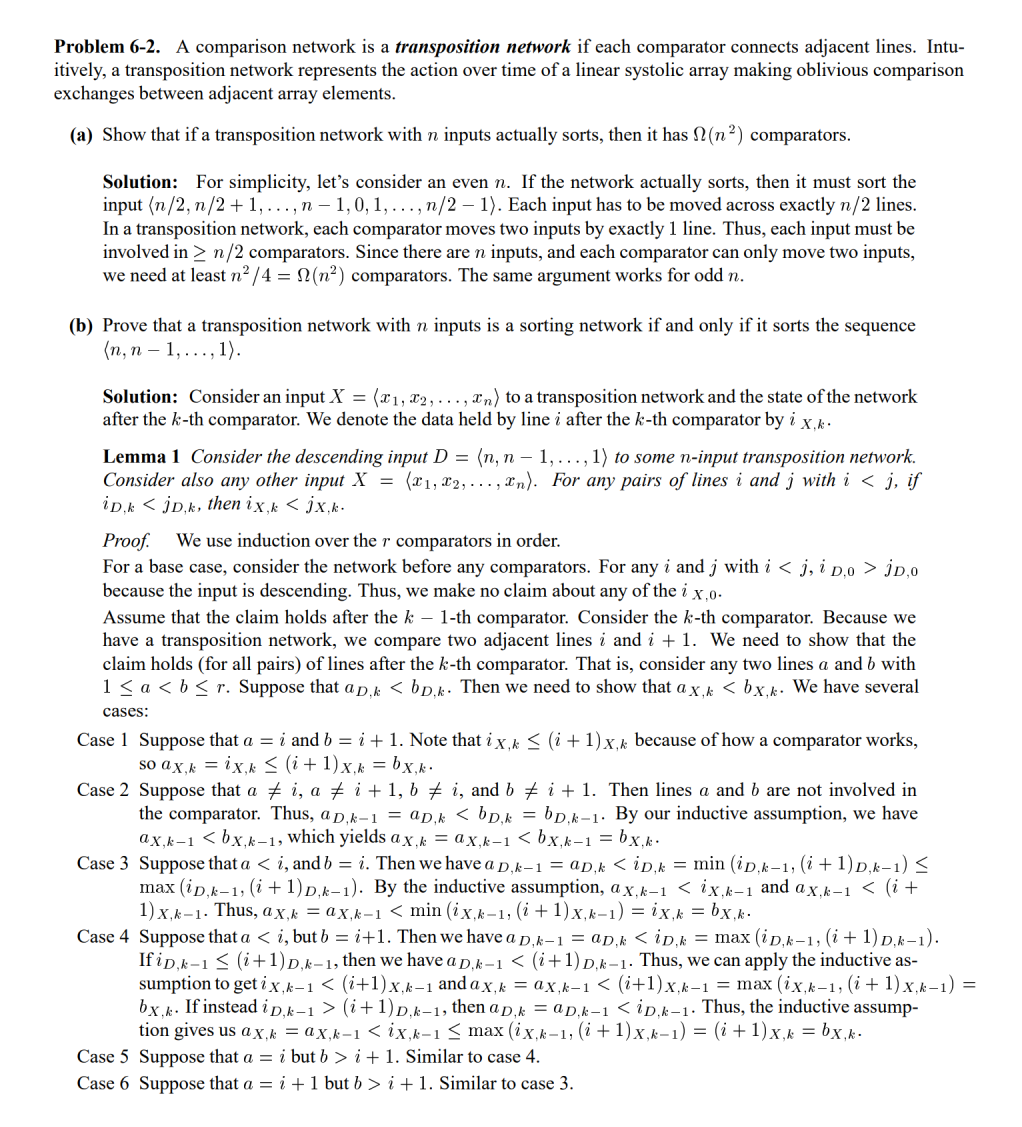
\includegraphics[width=0.6\textwidth]{rigorous_solution.PNG}
    \caption{The Rigorous Proof for Problem 3}\label{solution}
\end{figure}
%========================================================================
\end{document}
